\chapter{Ferramenta de Gestão de Requisitos}

“Para ser efetiva, a melhoria de processo de \textit{software} precisa contar com ferramentas que apoiem as atividades previstas nos processos. Sem a agilidade na execução, obtida por meio da adoção de ferramentas, as atividades que permitem visibilidade e controle dos processos podem se tornar um gargalo e, consequentemente, dificultar a institucionalização dos processos”.~\cite{mendes}

\section{Análise de ferramentas}

\subsection{IBM® Rational® RequisitePro}

O IBM Rational RequisitePro é uma ferramenta de gerenciamento de requisitos desenvolvida pela Rational Software, uma divisão dentro da IBM responsável pela elaboração de \textit{softwares} para auxiliar no desenvolvimento de um projeto. É uma ferramenta que permite gerenciar e rastrear os requisitos de negócio. 

Esta ferramenta é baseada no modelo iterativo incremental de desenvolvimento de \textit{software}, o RUP, que por sua vez é um modelo criado pela Rational Software. Ela unifica as duas abordagens da gerência de requisitos: a abordagem centrada a documentos e a centrada a banco de dados. Como o RequesitePro tem suporte nativo ao Microsoft Word®, ele consegue sincronizar um banco de dados comercial com esse programa, resultando na organização dos requisitos. Isso evita um repositório com documentos discordantes. Os principais pontos fortes encontrados na ferramenta, são a percepção automática da quebra de relacionamentos e a criação de visões da matriz de rastreabilidade. 

Alguns empecilhos para a utilização desta ferramenta são a sua compatibilidade apenas com a plataforma Windows e pelo fato de ser uma ferramenta paga, mesmo tendo um período de testes grátis, o \textit{trial}.

\begin{figure}[htb]
\centering
  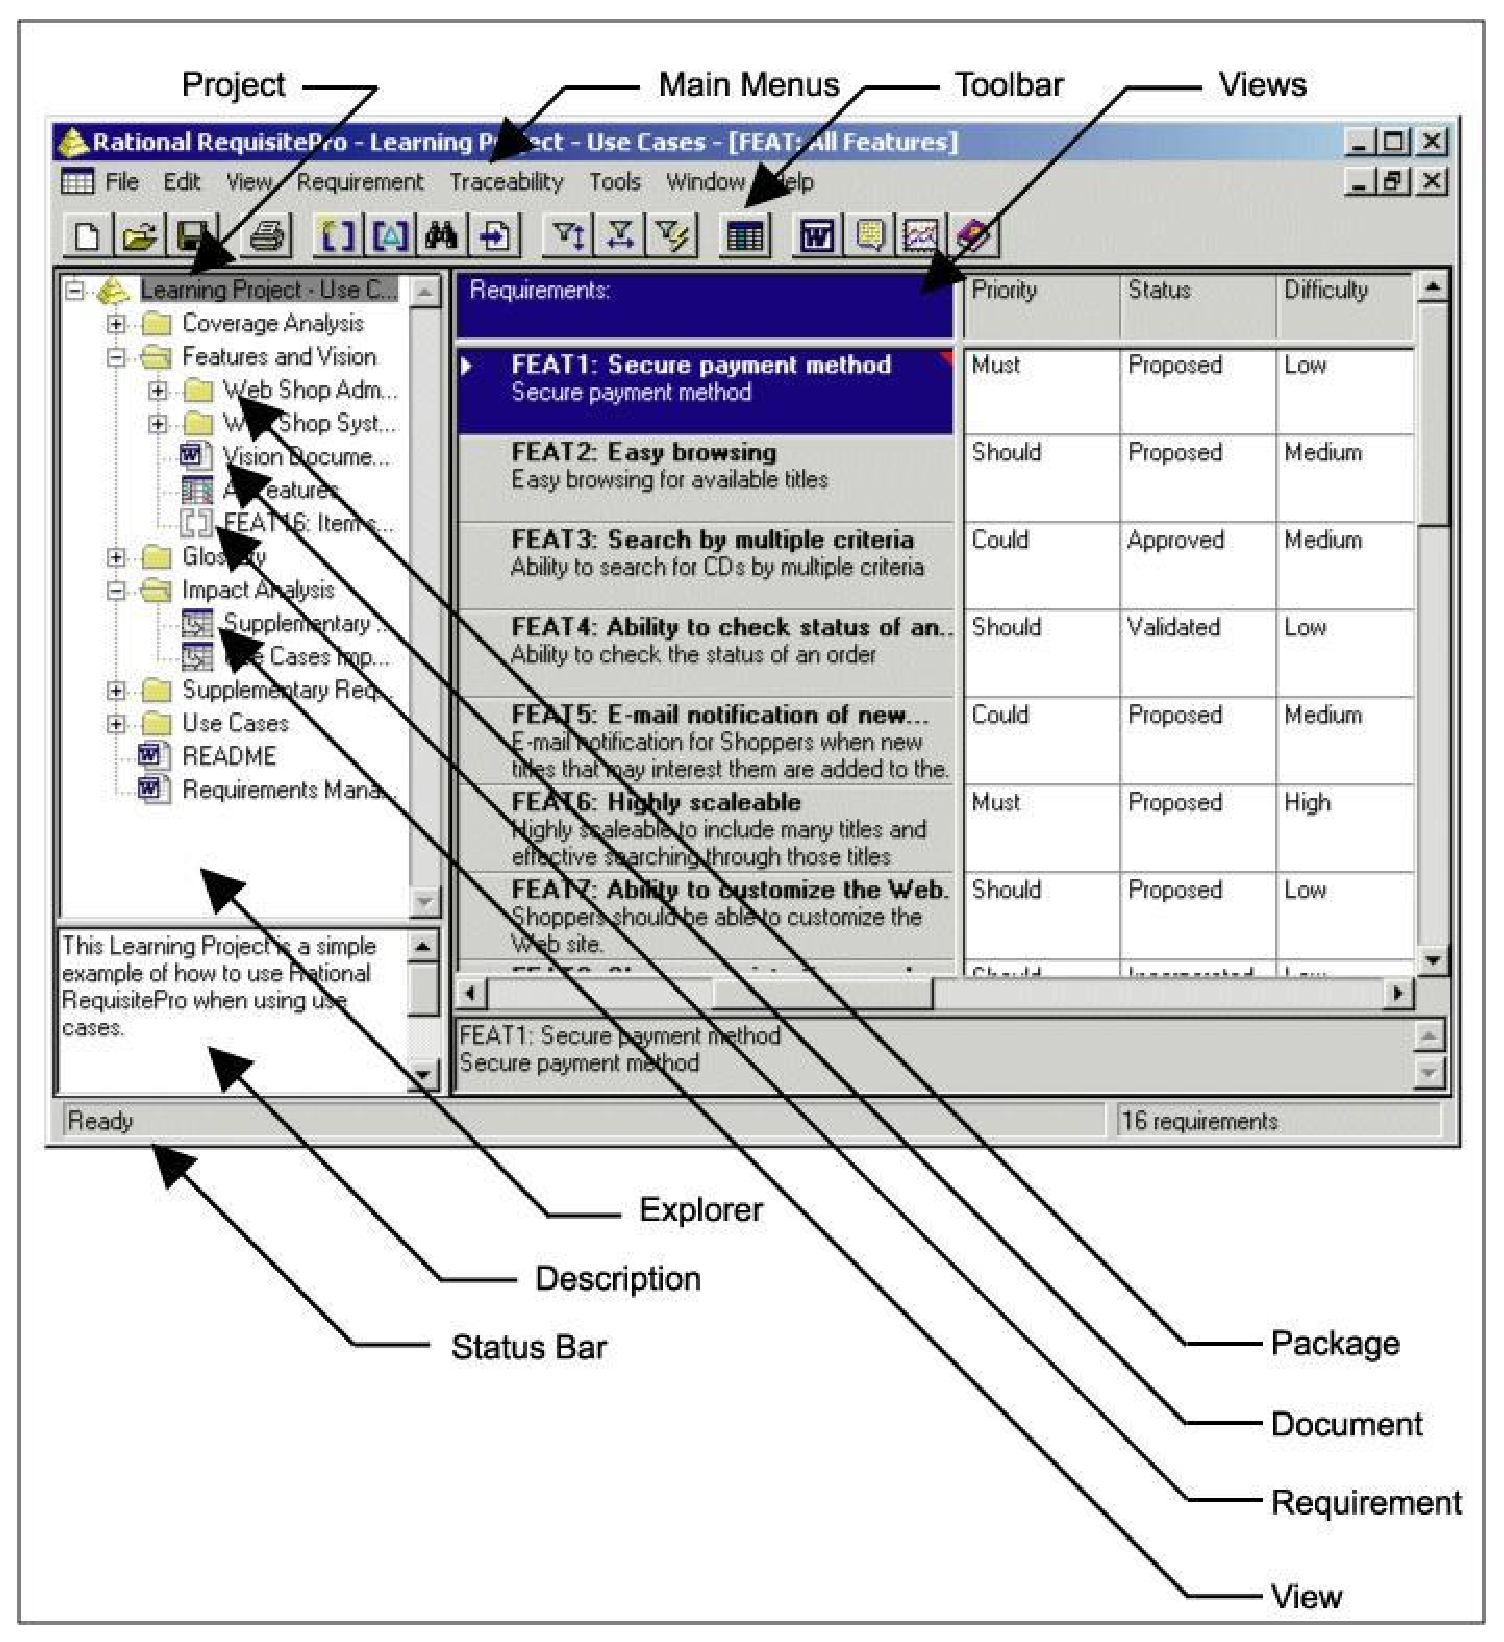
\includegraphics[keepaspectratio=true,scale=0.5]
  {figuras/requisit_pro.eps}
  \caption{Fonte: IBM/Rational (2006, p.146)}
  \label{requisit-pro}
\end{figure}

\clearpage{}

\subsection{Innoslate}

O Innoslate é uma ferramenta voltada ao ciclo de vida completo de um sistema, não apenas de gerenciamento de requisitos. Porém, em relação ao último uso, esse programa possui várias funções de auxílio.

Primeiramente ela nos possibilita facilmente editar e revisar os requisitos com uma janela de visualização de requisitos intuitiva. Assim como o Rational RequisitePro, o Innoslate nos permite importar os requisitos de outras plataformas como o Microsoft Word®, Microsoft Excel®, IBM® Rational® DOORS®, identificando e criando as relações pai/filho automaticamente. Uma outra \textit{feature} útil é a sua análise de requisitos, que exibe uma barra de qualidade para cada requisito, em porcentagem, além de dar sugestões para o seu aprimoramento. Há também outras funções auxiliares, não tão importantes como as anteriores, como gráficos hierárquicos, controle de versão e um ambiente customizável.

O Innoslate é uma ferramente paga, porém possui uma função que permite importar projetos. Somando isso ao período de 30 dias de teste (totalizando 120 dias para o time inteiro), não haverão problemas em sua utilização para o projeto. É importante, também, notar que se trata de uma ferramenta \textit{online}, impedindo assim eventuais incompatibilidades entre sistemas operacionais.

\begin{figure}[htb]
\centering
  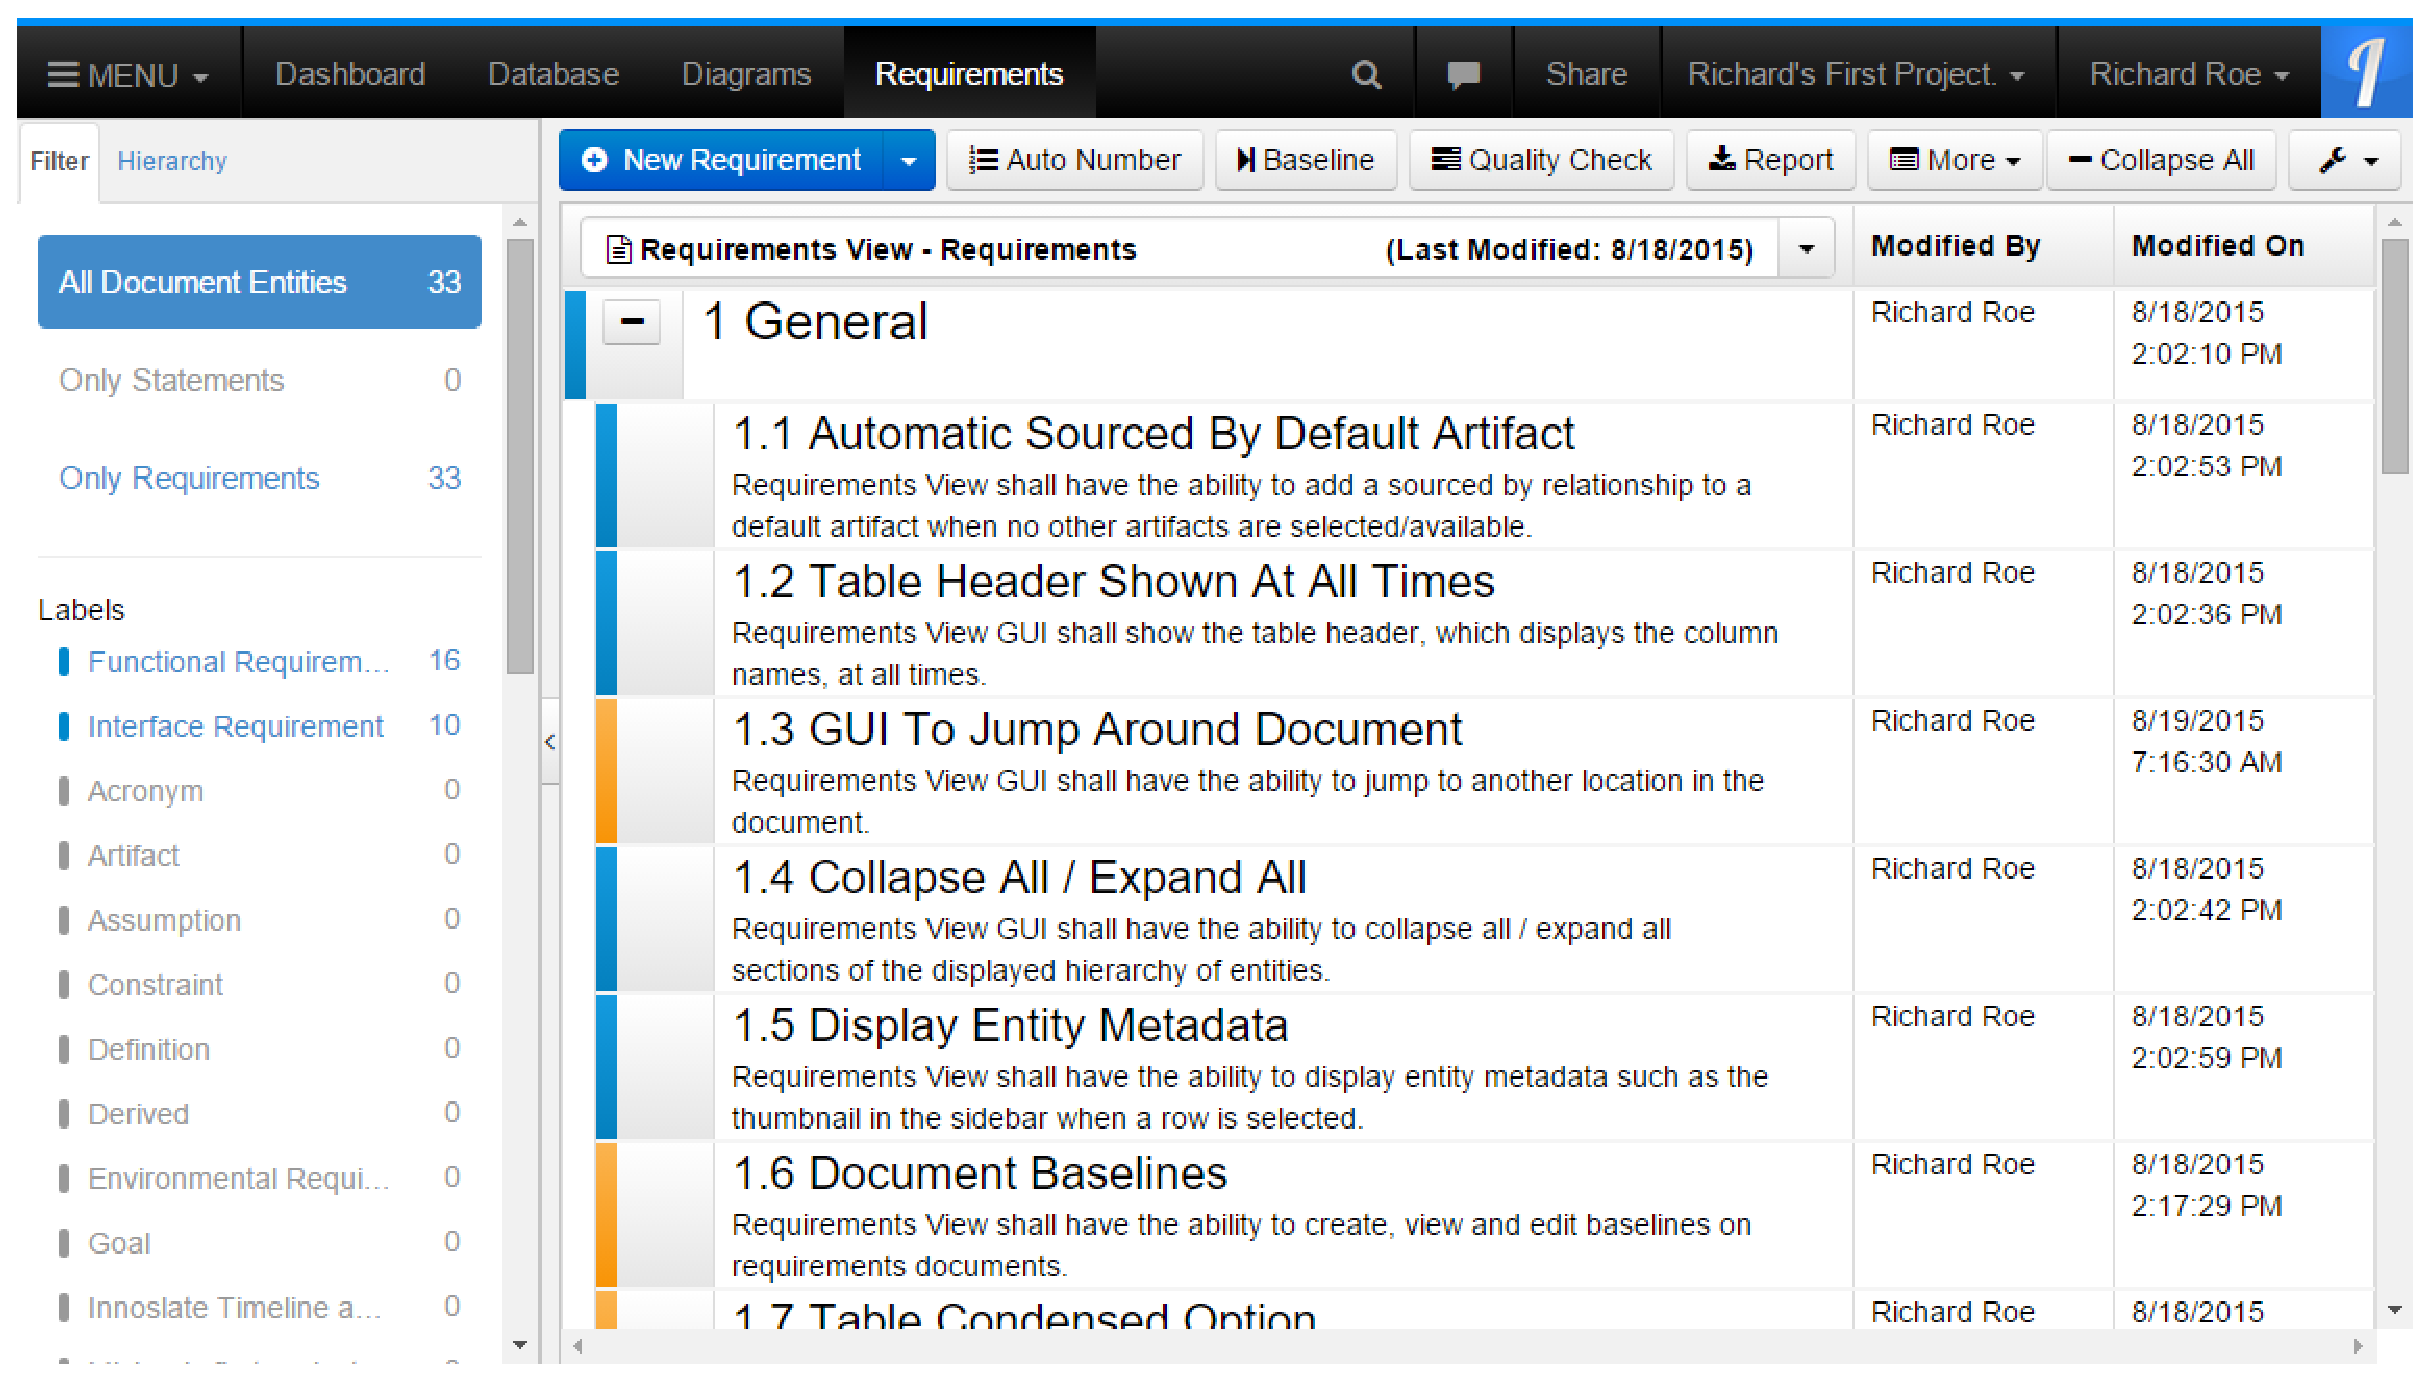
\includegraphics[keepaspectratio=true,scale=0.4]
  {figuras/innoslate.eps}
  \caption{Visualização de requisitos no Innoslate (Fonte: Innoslate User’s Guide)}
  \label{innoslate-pic}
\end{figure}

\clearpage{}

\subsection{Requirements One}

O Requirements One é uma ferramenta de gerência de requisitos voltada para a integração entre o time de desenvolvimento e os outros \textit{stakeholders}. Possui uma ampla gama de funcionalidades que permitem um bom gerenciamento de requisitos, além de possuir diversas integrações possíveis. As funcionalidades que destacam-se são: o seu modo de planejamento que permite que o gerente do projeto esteja a par de tudo que está acontecendo e seu sistema de \textit{issues} que facilita o entendimento da fonte da \textit{issue}, o que é de fundamental importância para a sua resolução com o menor tempo possível.

Esta ferramenta, como o Innoslate, é uma plataforma \textit{web} paga, também possuindo um período de testes. Possui uma interface agradável e alguns diferenciais interessantes, como \textit{wiki} e validação dos requisitos via \textit{feedback}.

\section{Critérios de avaliação}

Segundo ~\cite{beatty}, há uma série de atributos que devem ser analisados durante a escolha de uma ferramenta de gerenciamento de requisitos. Entre eles estão armazenamento de requisitos e seus atributos, rastreabilidade, usabilidade e gestão de mudanças. Dessa forma, as ferramentas foram julgadas tendo esses atributos como os critérios de escolha.

\begin{itemize}
\item Armazenamento de requisitos e seus atributos: Esta característica visa comparar a manutenção, análise e cadastro de requisitos.
\item Rastreabilidade: A partir dessa característica, pode-se comparar a maneira como os requisitos são organizados e se as ferramentas possuem funcionalidades para obter uma árvore de rastreabilidade.
\item Usabilidade: Com esta característica, foi analisado se as ferramentas forneciam uma boa experiência de uso, utilizando as boas práticas de interação humano-computador.
\item Gestão de mudanças: Esta é uma das características de maior destaque, pois busca verificar como os requisitos são modificados e fornecer uma visão da qualidade da elicitação.
\end{itemize}

Cada critério foi avaliado com uma nota inteira entre 0 (péssimo) e 10 (ótimo).

\begin{table}[]
\centering
\label{tools-performance}
\begin{tabular}{|l|l|l|l|}
\hline
Critério/Ferramenta                          & IBM Rational RequisitePro & Innoslate & Requirements One \\ \hline
Armazenamento                                & 8                         & 9         & 6                \\ \hline
Rastreabilidade                              & 6                         & 8         & 3                \\ \hline
Usabilidade                                  & 5                         & 8         & 10               \\ \hline
Gestão de Mudanças                           & 9                         & 7         & 6                \\ \hline
Total                                        & 28                        & 32        & 25               \\ \hline
\end{tabular}
\caption{Avaliação das ferramentas}
\end{table}

\section{Escolha da ferramenta}

Além das características de avaliação, a ferramenta deveria ser compatível com todos os sistemas operacionais utilizados no desenvolvimento. Também deve ser acessível, do ponto de vista financeiro. Levando em consideração essas últimas observações, a ferramenta escolhida foi a Innoslate por ser a que mais se destacou em relação aos critérios de avaliação.

